\documentclass{article}
\usepackage[utf8]{inputenc}


\usepackage{enumerate}
\usepackage{amsmath} % Tillater avansert formatering av matte.
\usepackage{amsfonts} % Tillater avanserte teikn, som R for reelle tall.
\usepackage{rotate, graphicx} % Tillater mer avansert formatering av grafikk.
\usepackage{geometry} % Tillater enklere formatering av sidevisning.
\usepackage{physics}
\usepackage{amssymb}
\usepackage{hyperref}
\usepackage{natbib}
\setlength\parindent{0pt}
\usepackage{listings}
\usepackage[dvipsnames]{xcolor}

\usepackage{color, colortbl}
\definecolor{yellow}{rgb}{255,255,0}
\definecolor{codegreen}{rgb}{0,0.6,0}
\definecolor{codegray}{rgb}{0.5,0.5,0.5}
\definecolor{codepurple}{rgb}{0.58,0,0.82}
\definecolor{backcolour}{rgb}{0.95,0.95,0.92}
 
\lstdefinestyle{mystyle}{
    backgroundcolor=\color{backcolour},   
    commentstyle=\color{codegreen},
    keywordstyle=\color{magenta},
    numberstyle=\tiny\color{codegray},
    stringstyle=\color{codepurple},
    basicstyle=\footnotesize,
    breakatwhitespace=false,         
    breaklines=true,                 
    captionpos=b,                    
    keepspaces=true,                 
    numbers=left,                    
    numbersep=5pt,                  
    showspaces=false,                
    showstringspaces=false,
    showtabs=false,                  
    tabsize=2
}

\lstset{style=mystyle}

\title{Project 2}
\author{Johanne Mehren, Marit Kollstuen, Stine Sagen}
\date{September 2018}

\begin{document}

\maketitle

\begin{abstract}
In this project we first implement Jacobi's method on a tridiagonal Toeplitz matrix to find its eigenvalues and corresponding eigenvectors.  Further, we study numerical solutions of the radial part of Schrodinger's equation in three dimensions. First for one electron that moves in a harmonic oscillator potential and then for two electrons. Jacobi's method proves to demand $\approx 1.5n^2$ rotations to diagonalize a matrix. In order to achieve a steady solution for the one-electron problem, one should use approximately $n = 250$ integration points and $\rho_{max} \approx 5$. The same value for $\rho_{max}$ is also applied to the two-electron case. Higher frequency $\omega_r$ reviles a higher probability of finding the electrons closer to the left corner of the radial coordinate axis. 
\end{abstract}


\section{Introduction}

This project is an attempt to develop an algorithm for solving eigenvalue problems of tridiagonal matrix systems. The Toeplitz matrix is a type of tridiagonal matrix, which has analytical eigenpairs. The algorithm applies Jacobi's method for solving eigenvalue problems, and will be thoroughly explained in the Theory section. We can then test the result of the algorithm compared to the analytic solutions by applying unit tests.

\medskip

The problems we are trying to solve are two-point boundary value problems of a spring fastened at both ends, which have analytical solutions, namely the Buckling Beam problem (Section \ref{sec:bbp}). We can exploit this property when developing the Jacobi algorithm in order to apply it on more complicated calculations. Later, we will use the same method in studying harmonic oscillator problems in three dimensions with one or two electrons.  This is a quantum mechanical problem that concerns the radial part of Schrodinger's equation (Equation \ref{eq:schr}) for one electron, which can be found in Section \ref{sec: oneelec}, and then for two electrons (Equation \ref{eq:schr2}), which can be found in Section \ref{sub:twoelec}.

\medskip

The Results and Discussion section (Section \ref{sec:res} and \ref{sec:conc}) contains the comparison of our calculations and the analytical results. The efficiency of our algorithm in terms of CPU time as well as number of rotations the algorithm requires are also considered. We are lastly discussing the ideal harmonic potential, $\rho_max$, and number of integration points, $n$, to obtain a stable solution for the one- and two electron problems. The code is written in Python version 3.6. 

\medskip

Our motivation for the project is to understand the advantages of solving differential equations by matrix operations. Since none of us are familiar with quantum mechanics, we use this project to learn more about other fields of physics and how we can implement this to boundary value problems in meteorology.  

\section{Theory}

\subsection{Orthogonal transformation} %% Task 2 a)

The main idea of orthogonal transformations is to rotate a vector about the origin and represent the same vector in a rotated coordinate system. Orthogonal transformations preserve the orthogonality of the obtained eigenvectors.  This can be shown by considering a basis of a vector $\textbf{v}_i$, where:

\[
\textbf{v}_i = 
\begin{bmatrix}
    v_{i1}&\\...&\\...&\\ v_{in}
\end{bmatrix}
\]

We assume that the basis is orthogonal, so that $\textbf{v}_j^T\textbf{v}_i = \delta_{ij}$. For an orthogonal (unitary) transformation, we have:  $\textbf{w}_i = \textbf{U}\textbf{v}_i$, in which $\textbf{U}$ is a unitary, orthogonal matrix so that $\textbf{U}^{-1} = \textbf{U}^T$ and $\textbf{U}^T\textbf{U} = \delta_{ij}$. The preservation of the dot product and orthogonality by unitary transformation of the vectors $\textbf{v}_i$ can then be shown by:

\begin{align*}
    \textbf{w}_i & = \textbf{U}\textbf{v}_i \\
    \textbf{w}_j^T\textbf{w}_i & = (\textbf{U}\textbf{v}_i)^T(\textbf{U}\textbf{v}_i) \\
    & = \textbf{v}_j^T\textbf{U}^T\textbf{U}\textbf{v}_i \\
    & = \textbf{v}_j^T \textit{\textbf{I}}  \textbf{v}_i \\
    & = \delta_{ij}
\end{align*}


\subsection{Jacobi's rotation method}
To solve the eigenvalue problem
\begin{equation}
    \mathbf{Au} = \lambda \mathbf{u}
    \label{eq:eigen}
\end{equation}
we can implement the Jacobi's rotation algorithm to a tridiagonal Toeplitz matrix. By applying the Jacobi rotation matrix $\textbf{S}_{kl}$:


\[
\textbf{S} = 
\begin{bmatrix}
    1 & 0 & ... & 0 & 0 & ... & 0 & 0 \\
    0 & 1 & ... & 0 & 0 & ... & 0 & 0 \\
    ... & ... & ... & 0 & 0 & ... & ... & ... \\
    0 & 0 & ... & \cos\theta & 0 & ... & 0 & \sin\theta \\
    0 & 0 & ... & 0 & 1 & ... & 0 & 0 \\
    ... & ... & ... & ... & ... & ... & 0 & ... \\
    0 & 0 & ... & 0 & 0 & ... & 1 & 0 \\
    0 & 0 & ... & -\sin\theta & 0 & ... & 0 & \cos\theta \\
\end{bmatrix}
\]

That contains ones along the diagonal except for two elements $\cos\theta$ in rows and columns $k$ and $l$. The off-diagonal elements are zero except the elements $\sin\theta$ and $-\sin\theta$. The matrix  $\textbf{S}_{kl}$ has the property $\textbf{S}^T = \textbf{S}^{-1}$. It performs a plane rotation around an angle $\theta$ until the matrix $\textbf{A}$ becomes almost diagonal, i.e. the non-diagonal elements are zero. The elements in the diagonal are approximations of the eigenvalues of $\textbf{A}$.

\subsection{The buckling beam problem}
The buckling beam problem can be visualized as a string with length $L, x \epsilon [0,L]$ fastened at both ends. This can be written as the differential equation

\begin{equation}
    \gamma \frac{d^2 u(x)}{dx^2} = -Fu(x)
    \label{eq:buckling}
\end{equation}

where $u(x)$ represents the vertical displacement of the beam in y-direction, the force $F$ applied at the beam towards origin and the parameter $\gamma$. Introducing the dimensionless variable $\rho = x/L, \quad \epsilon [0,1]$, rewrite Equation \ref{eq:buckling} and discretize, the problem can be written as an eigenvalue problem. We can apply this theory to problems in quantum mechanics as described in the two next subsections.  

\subsection{One electron in three dimensions}
\label{sec: oneelec}
According to \cite{electrons} few one-electron problems in quantum mechanics can be solved analytically . We will now consider a system with Coulomb correlations which has an exact solution by first evaluating one single electron in three dimension. The electron has a harmonic oscillator potential. The radial part of Schrodinger's equation in spherical coordinates can be written as 

\begin{equation}
    -\frac{\hslash^2}{2m}\Big(\frac{1}{r^2}\frac{d}{dr}r^2\frac{d}{dr}-\frac{1(l+1)}{r^2}\Big)R(r) + V(r)R(r) = ER(r)
    \label{eq:schr}
\end{equation}

In which $V(r)$ is the harmonic oscillator potential, $(1/2)kr^2$ with $k = m\omega^2$ and $E$ is the energy of the harmonic oscillator in three dimensions.

\medskip

Let $\omega$ be the oscillator frequency and $l$ represents the orbital momentum of the electron, the associated energies of the system is given by the relation: 

\begin{equation}
E_{nl} = \hslash\omega\bigg(2n + l + \frac{3}{2}\bigg)
\end{equation}
where $n = 0,1,2,...$ and $l= 0,1,2,...$

\medskip

Performing the substitution $R(r) = \frac{1}{r}u(r)$ and introducing a dimensionless variable $\rho = (\frac{1}{\alpha})r$ Equation (\ref{eq:schr}) now reads: 
\begin{equation}
    -\frac{\hslash^2}{2m\alpha^2}\frac{d^2}{d\rho^2}u(\rho) + \Big(V(\rho) + \frac{l(l+1)}{\rho^2}\frac{\hslash^2}{2m\alpha^2}\Big)u(\rho) = Eu(\rho)
    \label{eq:schr2}
\end{equation}
which has boundary conditions $u(0) = 0, u(\infty)=0$. Using a dimensionless variable $\rho$ makes it simple to implement the harmonic oscillator potential to our matrix. 

\medskip

Throughout this project, the orbital momentum $l$ is set to zero. Making this assumption, one can easily achieve the desirable eigenvalue problem to be studied closer. 

\medskip

Further, by substituting an expression for the harmonic oscillator potential $V(\rho) = \frac{1}{2}k\alpha^2\rho^2$ into Equation (\ref{eq:schr2}) and preform some multiplication and rearranging, the final Schrodinger's equation to be discretized now reads:

\begin{equation}
-\frac{d^2}{d\rho^2}u(\rho) + \rho^2u(\rho) = \lambda u(\rho)
\label{eq: schr3}
\end{equation}

Where $\lambda = \frac{2m\alpha^2}{h^2}E$ represents the eigenvalues.

\medskip

Applying the finite difference approximation obtained from Taylor expansion on the second order derivative, Equation (\ref{eq: schr3}) can be discretized as:
\begin{equation}
    -\frac{u_{i+1}-2u_{i} + u_{i-1}}{h^2} 
    + V_iu_i = \lambda u_i
\label{eq: schr_dis}
\end{equation}

With the harmonic oscillator potential defined as $V_i = \rho_i^2$

\medskip

The grid size is:
\begin{equation}
    h = \frac{\rho_N-\rho_0}{N}
\end{equation}

where N is the amount of grid points and $\rho_N$ and $\rho_0$ is the values taken at the boundary. 

\medskip

Equation (\ref{eq: schr_dis}) can be represented as a matrix eigenvalue problem (see Equation \ref{eq:eigen}) on the same form as the buckling beam problem.

\[
\begin{bmatrix}
	d_0 & e_0 & 0 & 0 & ... & 0 & 0 \\
	e_1 & d_1 & e_1 & 0 & ... & 0 & 0 \\
	0 & e_2 & d_2 & e_2 & 0 & ... & 0 \\
	... & ... & ... & ... & ... & ... & ... \\
	0 & ... & ... & ... & e_{N-1} & d_{N-1} & e_{N-1} \\
	0 & ... & ... & ... & ... & e_N & d_N
\end{bmatrix}
\begin{bmatrix}
	u_0 \\  u_1 \\ ... \\ ... \\ ... \\ u_N  
\end{bmatrix}
= \lambda
\begin{bmatrix}
    u_0 \\  u_1 \\ ... \\ ... \\ ... \\ u_N
\end{bmatrix}
\]


The diagonal and non-diagonal matrix elements are defined as $d_i = \frac{2}{h^2}+V_i$ and $e_i = -\frac{1}{h^2}$. The harmonic oscillator potential $V_i$ is thus added to the diagonal elements.

\subsection{Two electrons in three dimensions}
\label{sub:twoelec}

Adding an additionally electron to the potential oscillator yields a new issue to study. Two different cases are taken into account; one without Coulomb interaction and another where this interaction is present.  

\medskip

Schrodinger's Equation (\ref{eq:schr}) when there is no Coulomb interaction is now:
\begin{equation}
\bigg(-\frac{\hslash^2}{2m}\frac{d^2}{dr_1^2}-\frac{\hslash^2}{2m}\frac{d^2}{dr_2^2}+ \frac{1}{2}kr_1^2 + \frac{1}{2}kr_2^2\bigg)u(r_1,r_2) = E^{(2)}u(r_1,r_2)
\label{eq:schr2}
\end{equation}
$E^{(2)}$ is the total energy of the system,$E^{(2)} = E_r + E_R$, where $E_r$ is the relative energy and $E_R$ is the center-of-mass energy. The energies must be quantized as we are looking at a quantum mechanic system with confined electrons.  Since the solution of the center of mass is well known, we focus on the relative part. 

\medskip

When there is acting a repulsive Coulomb interacting given as:

\begin{equation}
V(r_1,r_2) = \frac{\beta e^2}{r}
\end{equation}
where $ \beta e^2 = 1.44$ eVnm.
This term can then be added to the Schrodinger's equation. Following the same procedure as for the one-electron case in which a dimensionless variable $\rho = \frac{r}{\alpha}$ is introduced and preform some rewriting, the Schrodinger's equation for two electrons case as an eigenvalue problem reads:

\begin{equation}
    -\frac{d^2}{d\rho^2}\psi(\rho) + \omega_{r}^2\rho^2\psi(\rho) + \frac{1}{\rho} = \lambda\psi(\rho)
\end{equation}

where the frequency parameter $\omega_r{}$ indicates the magnitude of the oscillator potential. 

\medskip

The harmonic oscillator potential in this case is $\omega_r^2\rho^2 + \frac{1}{\rho}$ in which are to be added to the diagonal. 

\medskip 


\section{Results}\label{sec:res}

\subsection{The buckling beam problem}\label{sec:bbp}

The Jacobi method was executed with a tolerance of $1E-8$ (i.e. iterations proceeded until all non-diagonal elements were lower than the tolerance and basically zero). Table \ref{tab:1} displays the iterations needed for the Jacobi method to converge for a given matrix of size $n\cross n$.  From the table, one can read that the iterations required for $n = 3$ is larger than for $n = 4$, and increasing thereafter. In general, The CPU-time (to the right) for small $n$ is also varying, but steadily increasing after $n = 50$.

\begin{table}[h]
\begin{tabular}{lll}
\hline
\textbf{Size of matrix ($n$):} & \textbf{Number of iterations:} & \textbf{CPU - time (sec):} \\ \hline
3                             & 10                            & 0.363                     \\
4                             & 7                             & 0.500                     \\
10                            & 154                           & 0.392                     \\
50                            & 4349                          & 0.519                     \\
100                           & 17660                         & 0.624                     \\
200                           & 70833                         & 4.01                      \\
300                           & 160140                        & 19.09               \\     
\hline
\end{tabular}
\label{tab:1}
\caption{Number of similarity transforms (iterations) required to achieve (near) zero-elements on the non-diagonals of a matrix of size $n\cross n$. CPU-time is given to the right}
\end{table}

\subsubsection{Unit test}

The unit test of the jacobi method is given below. Here, we are testing whether the eigenvalues yielded are the correct ones. This is done by checking if the eigenvalues yielded by the Jacobi method is the same as the ones calculated analytically and by the \texttt{numpy.linald.eig} method. 

\lstinputlisting[language=Python]{test_jacobi.py}

\subsection{One electron in three dimensions}

The code from the Buckling-beam problem was modified by adding the harmonic oscillator potential $\rho^2$ to the tridiagonal Toepliz matrix. Table \ref{fig:txt} shows the first four eigenvalues for different $n$ and $\rho_{max}$ = 5. The line highlighted in yellow is the best approximation out of the tests in which $\lambda_1 \approx 3$, $\lambda_2 \approx 7$, $\lambda_2 \approx 11$ and $\lambda_4 \approx 15$. With $n = 250$ integration points, we get similarity down to the fourth decimal for $\lambda_1$, $\lambda_2$ ad $\lambda_3$, and to the third decimal for $\lambda_4$.


\begin{table}[h]
\begin{tabular}{lllllll}
\centering
\hline
\textbf{$n$:} & \multicolumn{4}{l}{\textbf{Eigenvalues: $\lambda_1$, $\lambda_2$, $\lambda_3$ and $\lambda_4$:}} & \textbf{CPU (sec):} & \textbf{Iterations:} \\ \hline
10                                & 2.91948                  & 6.58303                  & 9.93656                   & 12.91647                  & 0.40344                  & 131                  \\
100                               & 2.99922                  & 6.99609                  & 10.99060                  & 14.98654                  & 0.82953                  & 16532                \\
200                               & 2.99980                  & 6.99903                  & 10.99778                  & 15.00057                  & 3.76951                  & 66618                \\ \rowcolor{yellow}
250                               & 2.99988                  & 6.99938                  & 10.99864                  & 15.00233                  & 8.25963                  & 104261               \\
300                               & 2.99991                  & 6.99957                  & 10.99912                  & 15.00331                  & 16.45377                 & 150728               \\
350                               & 2.99994                  & 6.99968                  & 10.99940                  & 15.00391                  & 30.23667                 & 205634               \\
400                               & 2.99995                  & 6.99976                  & 10.99958                  & 15.00431                  & 51.26365                 & 269129               \\ \hline
\end{tabular}
\caption{Tests for different integration points, $n$. The line highlighted in yellow is the best approximation of the eigenvalues $\lambda_1$, $\lambda_2$, $\lambda_2$ and $\lambda_4$. The CPU-time and number of rotations are listed to the right.}
\label{fig:txt}
\end{table}


\subsection{Two electrons in three dimensions}

The code from the Buckling-beam problem was modified by adding the oscillator potential $\omega_r^2\rho^2 + 1/\rho$ to the tridiagonal Toepliz matrix. In order to investigate stable results as functions of $\rho_{max}$, we use $\rho_{max} = 5$, that proved to be stable in the previous problem. 

\medskip

Figure \ref{fig:1} in Appendix \ref{appendix} displays the different radial wave functions for different $\omega$ with $\rho_{max} = 5$ and $n = 250$. Increasing the frequency $\omega$, it can be shown from the plot that the radial distance between the ground state becomes shorter and shorter. The red curve shows the largest value of $\omega_r$ when it takes the value $5$, and it is approaching zero at $\rho = 1$ compared to the blue curve for the lowest frequency which cover almost the whole range from $0$ to $5$.

\section{Discussion and conclusion}\label{sec:conc}

According to \cite{CompPhys}, one needs typically $3n^2$ to $5n^2$ rotations by the Jacobi method for the method to converge. However, from our results in Table \ref{tab:1}, the method converges after a bit less than approximately $1.5n^2$ iterations. The reason for the higher required number of iterations for $n = 3$ is not obvious to us, but afterwards the required number of iterations are steadily increasing, which is expected. 

\medskip

Table \ref{fig:txt} reveals that the best approximation to the analytic with scaling for the one-electron energies is achieved with $n \approx 250$ integration points and $\rho_{max} \approx 5$. From $n = 200$ to $n = 400$ integration points, the results have a closeness to the analytic results down to the fourth decimal for three out of four of the four first analytical eigenvalues, but fails to reproduce the third or the fourth.  

\medskip

When looking at Figure \ref{fig:1} in Appendix \ref{appendix} which displays the case for the two electrons, it is of interest how the wave function varies with different $\omega_r$. Increasing the value of $\omega_r$ results in higher peaks, but on the other hand the width is decreasing. Since the wave function $\abs{\phi(\rho)}^2$ is plotted, a probability distribution is present. According to Section \ref{sub:twoelec}, increasing of $\omega_r$ results in a stronger oscillator potential. The likelihood of finding the electrons closer to $\rho = 0$ can be deduced. 

\medskip

For future work one can let the orbital momentum $l$ differ from zero. This would make the solution to equation \ref{eq:schr} more complicated, but would be crucial in further understanding of quantum mechanic systems. We would also investigate why our Jacobi method converges after fewer rotations than the method provided by \cite{CompPhys}.

\medskip


\section{Documentation}

The material used in this project can be found in the group member's repository in GitHub:

\url{https://github.com/marikoll/FYS4150_projects/tree/master/project_2}

The Python 3.6 algorithm for the main program is located at: 

\url{https://github.com/marikoll/FYS4150_projects/blob/master/project_2/python/jacobi.py}

The Python 3.6 algorithm for the unit-test is located at: 

\url{https://github.com/marikoll/FYS4150_projects/blob/master/project_2/python/test_jacobi.py}

\newpage
\bibliographystyle{apalike}
\bibliography{literature.bib} 

\newpage
\appendix
\section{Appendix}

\label{appendix}


\begin{figure}[!H]
    \centering
    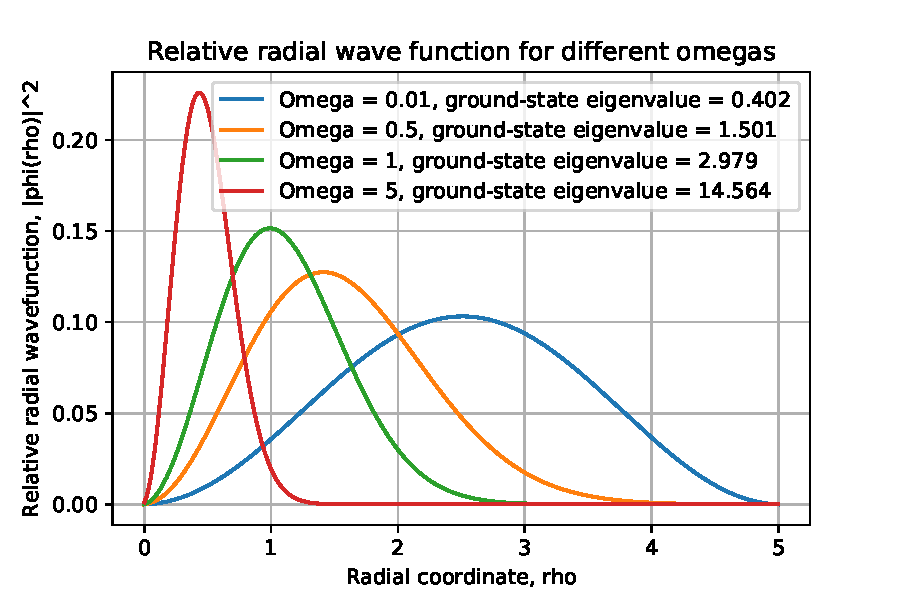
\includegraphics[width =\linewidth]{solutions.pdf}
    \caption{Plot of the radial wave function of four different frequencies ($\omega_r = 0,01,\omega_r = 0.5, \omega_r = 1$ and $\omega_r = 5)$ against the radial coordinate $\rho$, with $\rho_{max}$ chosen to be $\approx 5$ in order to reveal stable solutions. The number of grid points is $n = 250$. In addition to the values of $\omega$, the different values of the corresponding eigenvalues at ground state are also indicated in the label.}
    \label{fig:1}
\end{figure}

\end{document}

